\documentclass[xcolor=dvipsnames]{beamer}
\usepackage{beamerthemesplit}
%\usepackage{natbib}
\usepackage{bm,amsmath,color}
\definecolor{darkblue}{rgb}{0.0,0.0,0.50}
\definecolor{myorange}{cmyk}{0,0.7,1,0}
\hypersetup{colorlinks = true, linkcolor=darkblue, citecolor=darkblue, 
urlcolor=darkblue}
\hypersetup{pdfauthor={A. Richards}, pdftitle={Phylogenetic models and the DP}}

%% links
%\let\oldcite=\cite                                                              
%\renewcommand{\cite}[1]{darkblue}{\oldcite{#1}}}
%\renewcommand{\cite}[1]{\textcolor[rgb]{0.0,.7,1.0}{\oldcite{#1}}}

\newcommand{\rd}{\textcolor {red}}
\newcommand{\highlt}{\textcolor {myorange}}
\def\ci{\perp\!\!\!\perp}
%% set beamer theme and color
\usetheme{Frankfurt}
%\usecolortheme{dolphin}
\usecolortheme{rose}
\setbeamertemplate{blocks}[rounded][shadow=true]

%% beamer packages
% other themes: AnnArbor, Antibes, Bergen, Berkeley, Berlin, Boadilla, boxes, 
% CambridgeUS, Darmstadt, Dresden, Frankfurt, Goettingen, Hannover, Ilmenau,
%JuanLesPins, Luebeck, Madrid, Malmoe, Marburg, Montpellier, PaloAlto,
%Pittsburgh, Rochester, Singapore, Szeged, Warsaw
% other colors: albatross, beaver, crane, default, dolphin, dove, fly, lily, 
%orchid, rose, seagull, seahorse, sidebartab, structure, whale, wolverine,
%beetle
\title[Discussion]{Phylogenetic modeling\\ and the Dirichlet process}
\author[Richards]{Adam J. Richards}
\institute{Centre national de la recherche scientifique (CNRS) \ \\ \
(French National Center for Scientific Research) \ \\ \ Station
d'Ecologie Exp\'erimentale du CNRS \`a Moulis}
\date[\today]{Last updated: \today}

%%%%%%%%%%%%%%%%%%%%%%%%%%%%%%%%%%%%%%%%%%%%%%%%%%%%%%%%%%%%%%%%%%%%%%%%%%%%%%%
\begin{document}
\frame{\titlepage}
%%%%%%%%%%%%%%%%%%%%%%%%%%%%%%%%%%%%%%%%%%%%%%%%%%%%%%%%%%%%%%%%%%%%%%%%%%%%%%%
\frame{
\footnotesize
\tableofcontents
\normalsize
}
%%%%%%%%%%%%%%%%%%%%%%%%%%%%%%%%%%%%%%%%%%%%%%%%%%%%%%%%%%%%%%%%%%%%%%%%%%%%%%%
\section{Background}
\subsection{}
%%%%%%%%%%%%%%%%%%%%%%%%%%%%%%%%%%%%%%%%%%%%%%%%%%%%%%%%%%%%%%%%%%%%%%%%%%%%%%%
\frame{
\small
\begin{block}{Codon substitution models}
There are $4 \times 4 \times 4 = 64$ possible codons.  61 code for amino acids while the 3 others are stop codons.  So most amino acids are encoded by more than on codon allowing for substitutions in the genetic code that do not change the amino acid sequence (\highlt{synonymous}) substitutions. 
\end{block}
\begin{itemize}
 \item A major focus has been put on applying a \highlt{mechanistic} approach rather than \highlt{phenomenological} one \cite{Rodrigue10b}
 \item Generative models!
 \item Site-heterogeneity i.e. \cite{Rodrigue10a}  
\end{itemize}
\normalsize
}

%%%%%%%%%%%%%%%%%%%%%%%%%%%%%%%%%%%%%%%%%%%%%%%%%%%%%%%%%%%%%%%%%%%%%%%%%%%%%%%
\section{Dirichlet Process}
\subsection{}
 %%%%%%%%%%%%%%%%%%%%%%%%%%%%%%%%%%%%%%%%%%%%%%%%%%%%%%%%%%%%%%%%%%%%%%%%%%%%%%%
\frame{
 \begin{block}{Dirichlet Process}
  A stochastic process used in Bayesian nonparametric models of data. It is a distribution over distributions, where each draw
 from a Dirichlet process is itself a distribution
 \end{block}
 
 \begin{itemize}
  \item Parametric function estimation (e.g. regression, classification)
  \item Nonparametric function estimation with Gaussian Processes
  \item Parametric density estimation (e.g. Gaussian mixture models)
  \item Bayesian nonparametric density estimation with DP
  \item Semiparametric modeling (e.g. GLMMs but with nonparametric noise and/or nonparametric random effects)
  \item Model selection/averaging (clustering, neuron spike sorting, topic modeling, computer vision) 
  \end{itemize}  
 \begin{tiny}
 \begin{flushleft}
  See \href{http://www.columbia.edu/~jwp2128/Teaching/E6892/papers/mlss2007.pdf}{a lecture on Dirichlet processes} by Yee Whye Teh for individual references
 \end{flushleft}
 \end{tiny}
}

%%%%%%%%%%%%%%%%%%%%%%%%%%%%%%%%%%%%%%%%%%%%%%%%%%%%%%%%%%%%%%%%%%%%%%%%%%%%%%%
\frame{
\begin{block}{Dirichlet Process (DP)}
Also known as the \highlt{Ferguson distribution} \cite{Ferguson73}. DP is a distribution over distributions and was motivated by Bayesian density estimation.
\end{block}
Suppose $H$ is a probability distribution, and $G$ is a random probability distribution, both with support in space $\mathbb{X}$. Then $G$ is distributed according to a DP with base distribution $H$, and precision parameter $\alpha > 0$, for all finite and measurable partitions of $\mathbb{X}$.
} 
 
%%%%%%%%%%%%%%%%%%%%%%%%%%%%%%%%%%%%%%%%%%%%%%%%%%%%%%%%%%%%%%%%%%%%%%%%%%%%%%%
\frame{
A \highlt{Dirichlet distribution} is a distribution over the $K$-dimensional probability simplex
\begin{equation}
 \Delta_{K} = \{ (\pi_{1},\ldots,\pi_{K}) : \pi_{k } \geq 0, \sum_{k} \pi_{k} = 1  \} 
\end{equation}
$(\pi_{1},\ldots,\pi_{K})$ is Dirichlet distributed, i.e.
\begin{equation*}
 (\pi_{1},\ldots,\pi_{K}) \sim \text{Dirichlet}(\alpha_{1},...,\alpha_{K})
\end{equation*}
with parameters $(\alpha_{1},...,\alpha_{K})$, if 
\begin{equation*}
 p(\pi_{1},\ldots,\pi_{K}) = \frac{\Gamma( \sum_{k} \alpha_{k} )}{\sum_{k}\Gamma(\alpha_{k)}} \prod^{n}_{k=1} \pi_{k}^{\alpha_{k}-1}
\end{equation*}
}

%%%%%%%%%%%%%%%%%%%%%%%%%%%%%%%%%%%%%%%%%%%%%%%%%%%%%%%%%%%%%%%%%%%%%%%%%%%%%%%
\frame{
\frametitle{Properties of Dirichlet distributions}
\begin{itemize}
\item \highlt{Agglomerative property}
\begin{align*}
 (\pi_{1},\ldots,\pi_{K}) &\sim \text{Dirichlet}(\alpha_{1},...,\alpha_{K})\\
 (\pi_{1}+\pi_{2},\pi_{3},\ldots,\pi_{K}) &\sim \text{Dirichlet}(\alpha_{1}+\alpha_{2},\alpha_{3},...,\alpha_{K})
 \end{align*}
Also, works for partitions of $\pi_{i}$
\item \highlt{Decimative property}
\begin{align*}
 (\pi_{1},\ldots,\pi_{K}) &\sim \text{Dirichlet}(\alpha_{1},...,\alpha_{K})\\
 (\pi_{1}\tau_{1},\pi_{2}\tau_{2},\ldots,\pi_{K}) &\sim \text{Dirichlet}(\alpha_{1}\beta_{1},\alpha_{2}\beta_{2},\ldots,\alpha_{K})
 \end{align*}
\end{itemize}
}

%%%%%%%%%%%%%%%%%%%%%%%%%%%%%%%%%%%%%%%%%%%%%%%%%%%%%%%%%%%%%%%%%%%%%%%%%%%%%%%
\frame{
\frametitle{DP parameters}
A DP has two parameters
\begin{itemize}
 \item \highlt{Base distribution} $H$ - like the mean of the DP
 \item \highlt{Strength parameter} $\alpha$ - like an inverse-variance of the DP
\end{itemize}

\begin{equation*}
 G \sim \text{DP}(\alpha,H)
\end{equation*}

And for any partition $(A_{1},\ldots,A_{K})$ of $\mathbb{X}$:

\begin{equation*}
 (G(A_{1}),\ldots,G(A_{k})) \sim \text{Dirichlet}(\alpha H (A_{1}),\ldots,\alpha H (A_{K}))
\end{equation*}

Note that the $H$ is sometimes referred to as $G_{0}$.
}

%%%%%%%%%%%%%%%%%%%%%%%%%%%%%%%%%%%%%%%%%%%%%%%%%%%%%%%%%%%%%%%%%%%%%%%%%%%%%%%
\frame{
\frametitle{Polya Urn Scheme}
\scriptsize
Let $\bm{\theta} = \{\theta_{1},\ldots,\theta_{N}\}$ be a sequence of random variables. Drawn independently from a DP
\begin{align*}
 \theta_{j} &\sim G \\
 G &\sim \text{DP}(\alpha,H)
\end{align*}
Then the posterior of $G$ is a DP with precision $\alpha + N$ and base distribution
\begin{equation*}
 \frac{\alpha}{\alpha+N} H + \frac{1}{\alpha+N} \sum_{j=1}^{N} \delta_{\theta_{j}}
\end{equation*}
where $\delta_{\theta}$ Dirac probability mass function, placing all mass at $\theta$. Given this $\alpha$ is
interpreted as a \textit{prior sample size}, or the strength of prior belief in the base measure $H$.

\highlt{Polya urn scheme} - generative construction for $\bm{\theta}$ identified by marginalizing w.r.t. $G$.  The scheme yields:
\begin{equation}
 p(\theta_{j}|\bm{\theta}_{1:j-1}) \propto \alpha H(\theta_{j}) + \sum_{k=1}^{j-1} \delta_{\theta_{k}} \label{eqn:polya-urn}
\end{equation}
Eqn~\ref{eqn:polya-urn} is positive where $\theta_{j}$ is the same as $\theta_{k}$ and they are clustered when the probabilities are identical. 
\begin{flushleft}
\begin{tiny}
\cite{Blackwell73}
\end{tiny}
\end{flushleft}
\normalsize
}

%%%%%%%%%%%%%%%%%%%%%%%%%%%%%%%%%%%%%%%%%%%%%%%%%%%%%%%%%%%%%%%%%%%%%%%%%%%%%%%
\frame{
\frametitle{Chinese restaurant process}
\small
\begin{itemize}
 \item Draw $\theta_{1}, \ldots, \theta_{N}$ from a Blackwell-MacQueen urn scheme
 \item They take on $K < N$ distinct values, say $\theta_{1}^{*},\ldots,\theta_{K}^{*}$
 \item This defines a partition of $1,\ldots,N$ into $K$ clusters, such that if $i$ is in
       cluster $k$ , then $\theta_{i} = \theta_{k}^{*}$.
 \item Random draws $\theta_{1}, \ldots, \theta_{N}$ from a Blackwell-MacQueen urn scheme
       induce a random partition of $1,\ldots,N$.
 \item The induced distribution over partitions is a \highlt{Chinese restaurant process}.
\end{itemize}
\begin{flushleft}
\begin{tiny}
\cite{Aldous85}
\end{tiny}
\end{flushleft}
\normalsize
}

%%%%%%%%%%%%%%%%%%%%%%%%%%%%%%%%%%%%%%%%%%%%%%%%%%%%%%%%%%%%%%%%%%%%%%%%%%%%%%%
\frame{
\frametitle{More, more, more}
\small
There are more details... but instead here are the appropriate references. 
\begin{itemize}
 \item \highlt{DP} - introduced by \cite{Ferguson73}, while \cite{Antoniak74} further developed DPs and introduced mixtures of DPs.
 \item \highlt{Blackwell-MacQueen urn scheme} - \cite{Blackwell73} showed the scheme is exchangeable.
 \item \highlt{Chinese restaurant process} see \cite{Aldous85}
 \item MCMC is the primary means to summarize posterior quantities in DP models see \cite{MacEachern94,Escobar95}
 \item An alternative representation of the DP is the stick-breaking construction \cite{Sethuraman94}
 \item \highlt{Hierarchical Dirichlet Processes} were first developed by \cite{Teh06}
 \end{itemize}
\normalsize
}

%%%%%%%%%%%%%%%%%%%%%%%%%%%%%%%%%%%%%%%%%%%%%%%%%%%%%%%%%%%%%%%%%%%%%%%%%%%%%%%
\frame{
\frametitle{But why the DP?}
\small
\begin{block}{Cardinality}
Particularly an issue for clustering problems.  Although \highlt{model selection} and \highlt{cross-validation} are viable approaches to determine cardinality there are situations where a solution with these methods is generally intractable 
\end{block}
\begin{itemize}
 \item \highlt{Bayesian model averaging} - does not specify cardinality but rather average over several
 \item i.e. use a prior over the set of possible $K$ clusters and let the data define a posterior
 \item difficult to interpret and computational limitations
\end{itemize}
\normalsize
}

%%%%%%%%%%%%%%%%%%%%%%%%%%%%%%%%%%%%%%%%%%%%%%%%%%%%%%%%%%%%%%%%%%%%%%%%%%%%%%%
\frame{
\scriptsize
\begin{block}{Gaussian mixture model (GMM)}
A probabilistic model that assumes data is generated from a mixture of a \highlt{finite} number of Gaussian distributions with unknown parameters.
\end{block}
\begin{columns}
\begin{column}{5cm}
\begin{itemize}
 \item assumes a covariance structure i.e. spherical, diagonal, full, and tied
 \item full covariance normally performs best though it is overfits on small datasets
 \item plot: iris dataset --- training data (dots), test data (crosses) 
 \end{itemize}
\end{column}
\begin{column}{5cm}
 \begin{center}
 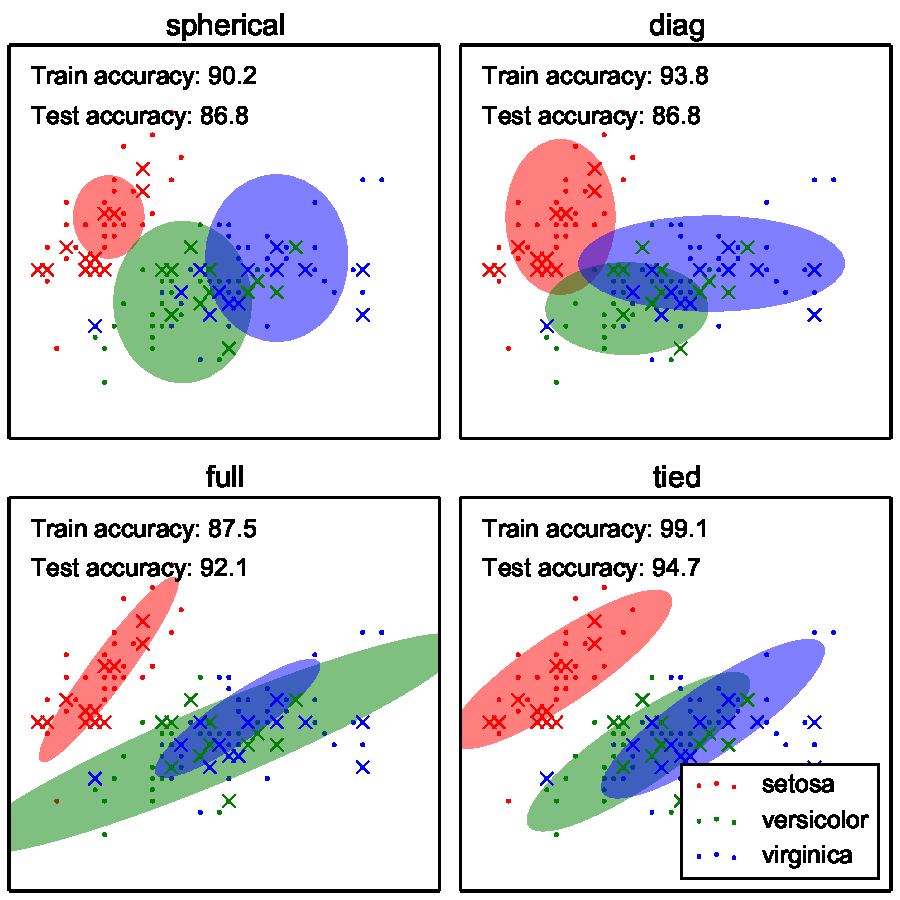
\includegraphics[scale = 0.32]{gmm_classifier_scikits.pdf} \\
 \end{center} 
\end{column}
\end{columns}
 \begin{tiny}
 \begin{flushleft}
  Modified from \href{http://scikit-learn.org/stable/auto_examples/mixture/plot_gmm_classifier.html}{scikit-learn documentation} 
 \end{flushleft}
 \end{tiny}
\normalsize
}

%%%%%%%%%%%%%%%%%%%%%%%%%%%%%%%%%%%%%%%%%%%%%%%%%%%%%%%%%%%%%%%%%%%%%%%%%%%%%%%
\frame{
\frametitle{GMMs continued}
\small
Different forms of inference exist:
\begin{itemize}
 \item Expectation-Maximization (EM)
    \begin{itemize}
       \item fast
       \item singularities (infinite likelihood)
       \item need to specify the number of components
    \end{itemize}
 \item Variational inference
    \begin{itemize}
       \item avoids singularities so we can use full covariance in high dimensions
       \item will bias all means towards the origin and covariances tend towards spherical
       \item need to specify hyperparameter (cross-validation)
    \end{itemize}
 \item MCMC
    \begin{itemize}
    \item exact solution upon convergence
    \item computational costly
    \end{itemize}
\end{itemize}
\normalsize
}

%%%%%%%%%%%%%%%%%%%%%%%%%%%%%%%%%%%%%%%%%%%%%%%%%%%%%%%%%%%%%%%%%%%%%%%%%%%%%%%
\frame{
\frametitle{Finite mixture models}
\begin{columns}
\begin{column}{5cm}
\begin{align*}
\theta^{*}_{k} &\sim H\\
\pi &\sim \text{Dirichlet}(\alpha/K, \ldots, \alpha/K)\\
z_{i}|\pi &\sim \text{Discrete}(\pi)\\
x_{i}|\theta^{*}_{z_{i}} &\sim F(\cdot|\theta^{*}_{z_{i}}) 
\end{align*}
Still have to use model selection/averaging over the hyperparameters in $H$, the Dirichlet parameter $\alpha$ and the number of components $K$
 \end{column}
\begin{column}{5cm}
\begin{center}
 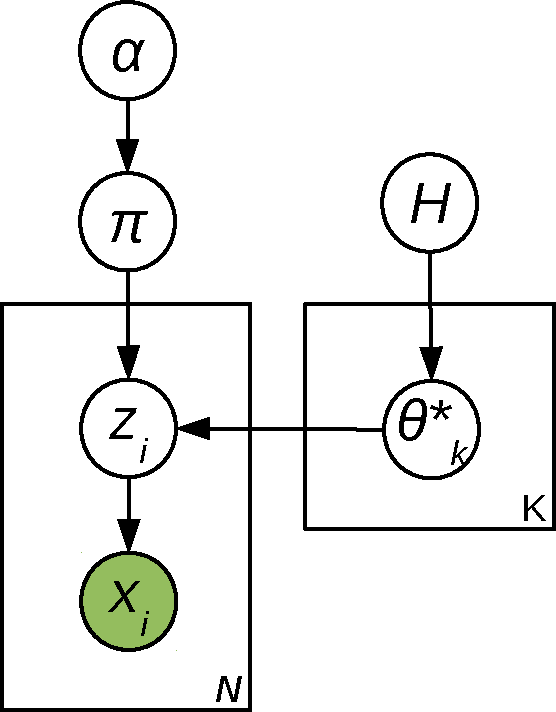
\includegraphics[scale=0.4]{bayesian-clustering.pdf}
\end{center}
\end{column}
\end{columns}
}

%%%%%%%%%%%%%%%%%%%%%%%%%%%%%%%%%%%%%%%%%%%%%%%%%%%%%%%%%%%%%%%%%%%%%%%%%%%%%%%
\frame{
\frametitle{Infinite mixture models}
\scriptsize
\begin{block}{}
Dirichlet Process Gaussian Mixture Model (DPGMM) --- an infinite mixture model with the Dirichlet Process as a prior distribution on the number of clusters. 
\end{block}
\begin{columns}
\begin{column}{5cm}
\begin{itemize}
 \item Let $K$ be very large
 \item If parameters $\theta_{k^{*}}$ and mixing proportions $\pi$
integrated out, the number of latent variables left does not grow with $K$ and we have no overfitting
 \item At most $N$ components will be associated with the data 
\end{itemize}
\end{column}
\begin{column}{5cm}
\begin{center}
 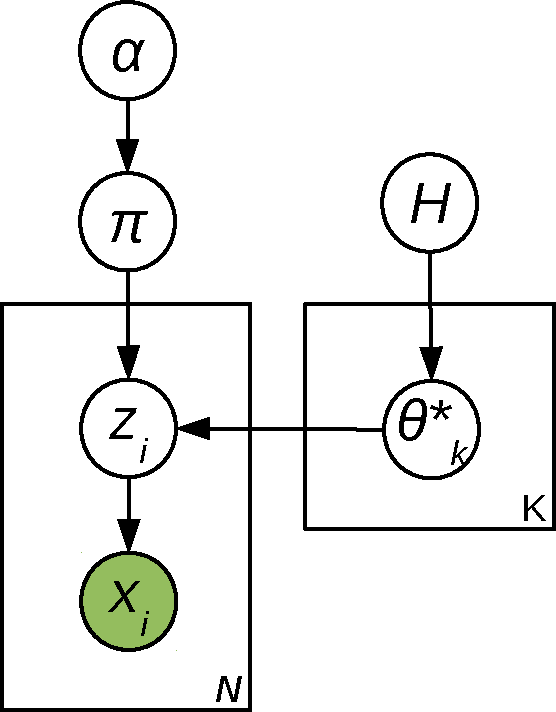
\includegraphics[scale=0.4]{bayesian-clustering.pdf}
\end{center}
\end{column}
\end{columns}

\begin{flushleft}
\begin{tiny}
The Infinite Gaussian mixture model \cite{Rasmussen00}
\end{tiny}
\end{flushleft}
\normalsize
}

%%%%%%%%%%%%%%%%%%%%%%%%%%%%%%%%%%%%%%%%%%%%%%%%%%%%%%%%%%%%%%%%%%%%%%%%%%%%%%%
\frame{
If we specify $K=5$...
\begin{center}
 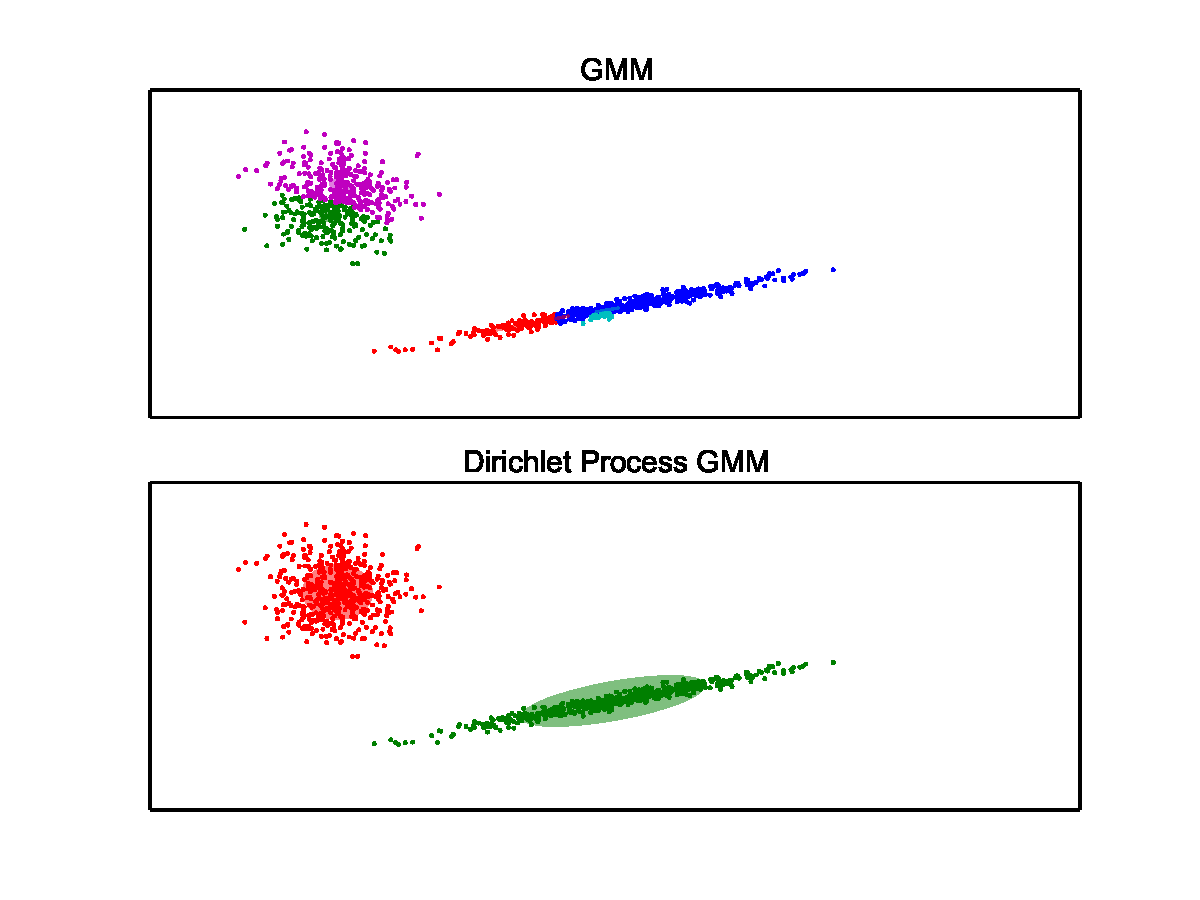
\includegraphics[scale=0.4]{dpgmm_example_scikit.pdf}
\end{center}
\begin{tiny}
 \begin{flushleft}
  Modified from \href{http://scikit-learn.org/stable/auto_examples/mixture/plot_gmm.html
}{scikit-learn documentation}. 
This model is implemented using variational inference as derived in \cite{Blei05}
\end{flushleft}
\end{tiny}
}

%%%%%%%%%%%%%%%%%%%%%%%%%%%%%%%%%%%%%%%%%%%%%%%%%%%%%%%%%%%%%%%%%%%%%%%%%%%%%%%
\frame{
\frametitle{a closer look at $\alpha$}
\small
\begin{center}
 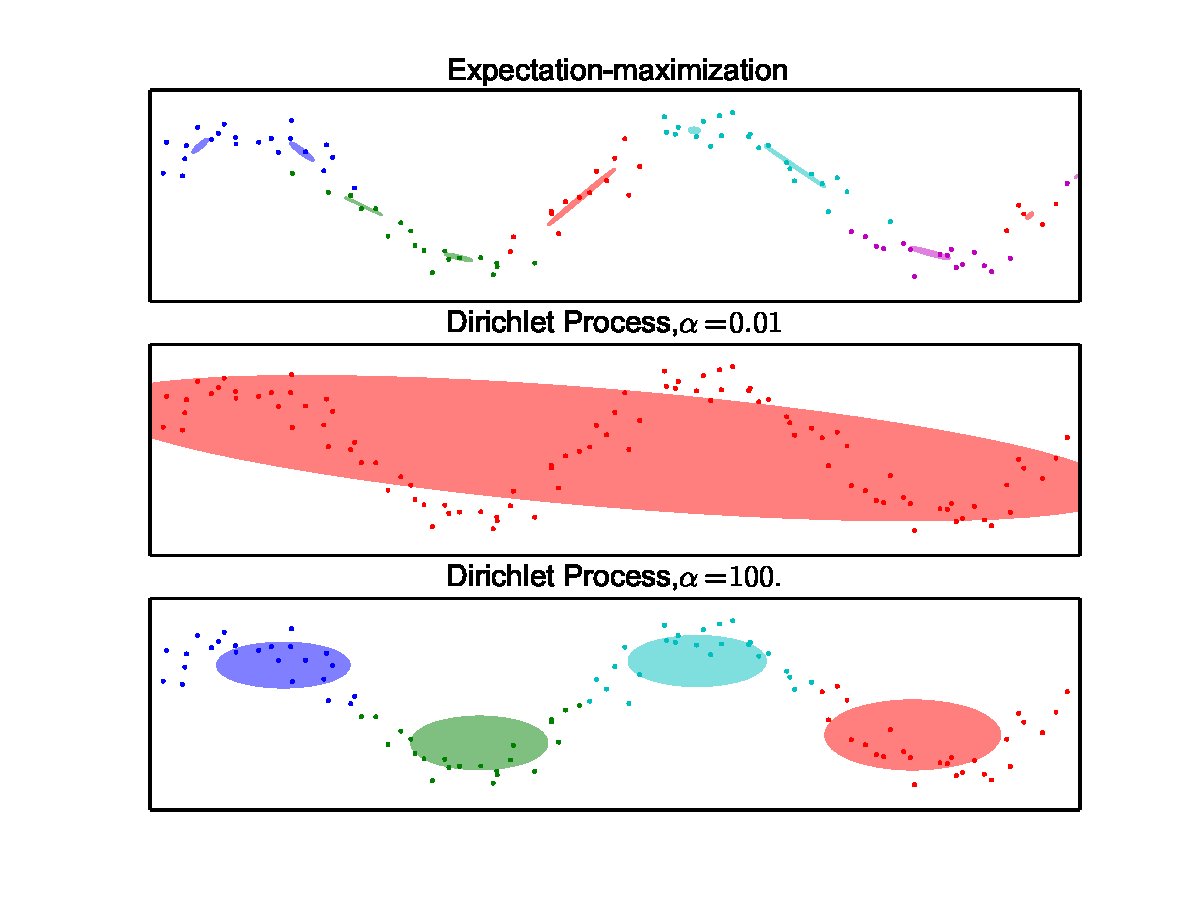
\includegraphics[scale=0.4]{dpmm_sin_example.pdf}
\end{center}
The strength parameter $\alpha$ acts like the precision (inverse variance) of the DP
\begin{tiny}
 \begin{flushleft}
  Modified from \href{http://scikit-learn.org/stable/auto_examples/mixture/plot_gmm_sin.html}{scikit-learn documentation} 
 \end{flushleft}
 \end{tiny}
\normalsize
 }

%%%%%%%%%%%%%%%%%%%%%%%%%%%%%%%%%%%%%%%%%%%%%%%%%%%%%%%%%%%%%%%%%%%%%%%%%%%%%%%
\section{CAT models}
\subsection{}
%%%%%%%%%%%%%%%%%%%%%%%%%%%%%%%%%%%%%%%%%%%%%%%%%%%%%%%%%%%%%%%%%%%%%%%%%%%%%%%
\frame{
\frametitle{CAT model}
\scriptsize
\begin{itemize}
 \item Relax the assumption that proteins evolve under the sample substitution process ($20 \times 20$ substitution matrix)
 \item AA replacement at different sites of a protein alignment can have distinct substitution processes
 \item CAT model assumes distinct processes (classes) differing by equilibrium frequencies over the 20 residues
 \item Using a DP the affiliations of each site to a given class are free variables
 \item Substitutional heterogeneity is estimated using posterior means (classes)
 \item Data come in the form on an alignment of $P$ amino acid sequences of length $N$.
 \item Substitutions occur according to a rate matrix $Q_{lm}$ expressed in terms of 20 probabilities or equilibrium frequencies.
\end{itemize}
\begin{flushleft}
  \tiny{\cite{Lartillot04}}
 \end{flushleft}
 \normalsize
}

%%%%%%%%%%%%%%%%%%%%%%%%%%%%%%%%%%%%%%%%%%%%%%%%%%%%%%%%%%%%%%%%%%%%%%%%%%%%%%%
\frame{ 
\frametitle{CAT continued}
\small
Let $\pi_{l}$ be the set of 20 equilibrium frequencies, s.t. $\sum^{20}_{l=1} = 1$.  And let $\rho_{lm}$ be the exchangeability parameters that are assumed to hold the relation,
\begin{align*}
Q_{lm} &= \frac{1}{Z} \rho_{lm} \pi_{m}, l \neq m \\
Q_{ll} &= -\sum_{m \neq l} Q_{lm}
\end{align*}
The process is assumed to be reversible $Q_{lm} = Q_{ml}$ and the matrix is scaled to 1 using the normalizing constant
\begin{equation}
 Z = 2 \times \sum_{1 \leq l \leq m \leq 20} \rho_{lm} \pi_{l} \pi_{m}
\end{equation}
\normalsize
\begin{flushleft}
  \tiny{\cite{Lartillot04}}
 \end{flushleft}
}

%%%%%%%%%%%%%%%%%%%%%%%%%%%%%%%%%%%%%%%%%%%%%%%%%%%%%%%%%%%%%%%%%%%%%%%%%%%%%%%
\frame{ 
\frametitle{CAT continued}
\small
Branch lengths are measured as the expected number of substitutions per site.  From $Q$ the transition probability matrix $P(v) = [P_{lm}(v)]$ can be used to specify the probability that amino-acid $l$ changes into $m$ over an evolutionary distance of $v$ via $P(v) = e^{vQ}$

Under the CAT model sites are distributed according to a mixture of $K$ distinct classes-- each class is characterized by its own substitution matrix $Q^{k}$.  An classes are specified using the vector $z$.  
\normalsize
\begin{flushleft}
  \tiny{\cite{Lartillot04}}
 \end{flushleft}
}



%%%%%%%%%%%%%%%%%%%%%%%%%%%%%%%%%%%%%%%%%%%%%%%%%%%%%%%%%%%%%%%%%%%%%%%%%%%%%%%
% \frame{
% \frametitle{2010 PNAS paper}
% 
% \begin{itemize}
%  \item Captures marginal site specificities induced by purifying selection, based on site-heterogeneous modeling of AA fitness
% \end{itemize}
%  \begin{flushleft}
%   \tiny{\cite{Yang08}}
%  \end{flushleft}
%  \normalsize
% }

%%%%%%%%%%%%%%%%%%%%%%%%%%%%%%%%%%%%%%%%%%%%%%%%%%%%%%%%%%%%%%%%%%%%%%%%%%%%%%%
\section{Other models}
\subsection{}
%%%%%%%%%%%%%%%%%%%%%%%%%%%%%%%%%%%%%%%%%%%%%%%%%%%%%%%%%%%%%%%%%%%%%%%%%%%%%%%
\frame{
\frametitle{Muse and Gaut Model (MG)}
\scriptsize
The following formulation, inspiried by Muse and Gaut, is a basic codon substitution model that has two sets of parameters.
\begin{align}
 \rho &= (\rho_{lm}) \text{ where } lm \in \{1 \ldots 4 \} \text{ and } \sum \rho_{lm} = 1 \\
 \varphi &= (\varphi_{m}) \text{ where } m \in \{1 \ldots 4 \} \text{ and } \sum \varphi_{m} = 1 
\end{align}

\begin{equation}
Q_{ab} = \left\{
\begin{array}{l l}
\rho_{a_{c} b_{c}},                        & \quad \text{\tiny{if a and b are synonymous and differ only at} } c^{\text{th}} \text{\tiny{codon position}}\\
\omega \rho_{a_{c} b_{c}} \varphi_{b_{c}}, & \quad \text{\tiny{if a and b are nonsynonymous and differ only at} } c^{\text{th}} \text{\tiny{codon position}}\\
0,                                         & \quad \text{\tiny{otherwise.}} 
\end{array} \right.
\end{equation}

\footnotesize
$a_{c}$ corresponds to the index of the nucleotide at the $c^{\text{th}}$ ($c \in \{1,2,3\}$) position of codon $a$.  Extensions to the model model also includes $\omega$, modulating nonsynonymous rates without regard to the amino acids involved (MG-NS) or instead of $\omega$ we can apply a Dirichlet process approach to capture across-site heterogeneity in nonsynonymous mutation rates (MG-NSDP).
\normalsize
\begin{flushleft}
 \tiny{\cite{Muse94}}
\end{flushleft}
}

%%%%%%%%%%%%%%%%%%%%%%%%%%%%%%%%%%%%%%%%%%%%%%%%%%%%%%%%%%%%%%%%%%%%%%%%%%%%%%%
\frame{
\frametitle{Yang and Nielsen (CP)}
\footnotesize
This approach, inspired by Yan and Nielsen, uses a set of 61 codon fitness parameters.
\begin{equation} 
 \psi = (\psi_{a}) \text{ where } a \in \{1 \ldots 61 \} \text{ and } \sum a = 1 
\end{equation}

\begin{equation}
 Q_{ab} = \left\{
 \begin{array}{l l}
 \rho_{a_{c} b_{c}} \varphi_{b_{c}} \left( \frac{\psi_{b}}{\psi_{a}} \right)^{1/2},                        
     & \quad \text{\tiny{if a and b are synonymous and differ only at} } c^{\text{th}} \text{\tiny{codon position}}\\
 \omega \rho_{a_{c} b_{c}} \varphi_{b_{c}} \left( \frac{\psi_{b}}{\psi_{a}} \right)^{1/2}, 
     & \quad \text{\tiny{if a and b are nonsynonymous and differ only at} } c^{\text{th}} \text{\tiny{codon position}}\\
    0,                                         
     & \quad \text{\tiny{otherwise.}} 
  \end{array} \right.
 \end{equation}
With or without $\omega$ the models are referred to as Codon Preference (CP).  Therefore we have MG-CP, MG-NS-CP, and MG-NSDP-CP.
\footnotesize
\begin{flushleft}
 \tiny{\cite{Yang08}}
\end{flushleft}
\normalsize
}

%%%%%%%%%%%%%%%%%%%%%%%%%%%%%%%%%%%%%%%%%%%%%%%%%%%%%%%%%%%%%%%%%%%%%%%%%%%%%%%
\frame{
 \frametitle{Robinson \textit{et al.} (SC)}
 \scriptsize
 Approach inspired by Robinson \textit{et al.} Rodrigue \textit{et al.} define a model in sequence space.  Rates are given from one sequence state $s$ to another $s’$.
 
\begin{equation}
 R_{SS'} = \left\{
 \begin{array}{l l}
 \rho_{s_{i_{c}} s'_{i_{c}}} \varphi_{s_{i_{c}}},                        
     & \quad \text{\tiny{if A}}\\
 \omega  \rho_{s_{i_{c}} s'_{i_{c}}} \varphi_{s_{i_{c}}} e^{\beta(G_{(s)} - G_{(s')})},\\
     & \quad \text{\tiny{if B}}\\
    0,                                         
     & \quad \text{\tiny{otherwise.}} 
  \end{array} \right.
\end{equation}

where $s_{i}$ is the codon at the $i^{\text{th}}$ site of sequence $s$ and $s_{i_{c}}$ is the nucleotide at the $c^{\text{th}}$ codon of the $i^{\text{th}}$ site of sequence $s$.
\begin{itemize}
\item[A] $s$ and $s'$ differ only only at $c^{\text{th}}$ codon position at the $i^{\text{th}}$ site (implies synonymous change)
\item[B] $s$ and $s'$ differ only only at $c^{\text{th}}$ codon position at the $i^{\text{th}}$ site (implies nonsynonymous change)
\end{itemize}

For a given sequence $s$, $G(s)$ returns a pseudo-energy score of sequence-structure compatibility (see \cite{Kleinman06}).  These are referred to as Structurally Constrained (SC) models. MG-SC, MG-NS-SC and MG-NSDP-SC.

 \begin{flushleft}
  \tiny{\cite{Robinson03,Rodrigue09a}}
 \end{flushleft}
 \normalsize
}

%%%%%%%%%%%%%%%%%%%%%%%%%%%%%%%%%%%%%%%%%%%%%%%%%%%%%%%%%%%%%%%%%%%%%%%%%%%%%%%
\frame{
 \frametitle{SC + CP}
 \scriptsize
 
\begin{equation} 
  \psi = (\psi_{i_{c}}) \text{ where } i_{c} \in \{1 \ldots 61 \} \text{ and } \sum i_{c} = 1 
\end{equation}
 
 
\begin{equation}
 R_{SS'} = \left\{
 \begin{array}{l l}
 \rho_{s_{i_{c}} s'_{i_{c}}} \varphi_{s_{i_{c}}} \left( \frac{\psi_{s'_{i}}}{\psi_{s_{i}}} \right)^{1/2},                        
     & \quad \text{\tiny{if A}}\\
 \omega  \rho_{s_{i_{c}} s'_{i_{c}}} \varphi_{s_{i_{c}}} \left( \frac{\psi_{s'_{i}}}{\psi_{s_{i}}} \right)^{1/2} e^{\beta(G_{(s)} - G_{(s')})},\\
     & \quad \text{\tiny{if B}}\\
    0,                                         
     & \quad \text{\tiny{otherwise.}} 
  \end{array} \right.
\end{equation}

where $s_{i}$ is the codon at the $i^{\text{th}}$ site of sequence $s$ and $s_{i_{c}}$ is the nucleotide at the $c^{\text{th}}$ codon of the $i^{\text{th}}$ site of sequence $s$.
\begin{itemize}
\item[A] $s$ and $s'$ differ only only at $c^{\text{th}}$ codon position at the $i^{\text{th}}$ site (implies synonymous change)
\item[B] $s$ and $s'$ differ only only at $c^{\text{th}}$ codon position at the $i^{\text{th}}$ site (implies nonsynonymous change)
\end{itemize}

These models are referred to as MG-CP-SC, MG-NS-CP-SC, and MG-NSDP-CP-SC.
 \begin{flushleft}
  \tiny{\cite{Rodrigue10b}}
 \end{flushleft}
 \normalsize
}

%%%%%%%%%%%%%%%%%%%%%%%%%%%%%%%%%%%%%%%%%%%%%%%%%%%%%%%%%%%%%%%%%%%%%%%%%%%%%%%
\frame{
 \frametitle{Model comparisons}
 \scriptsize

 \begin{center}
 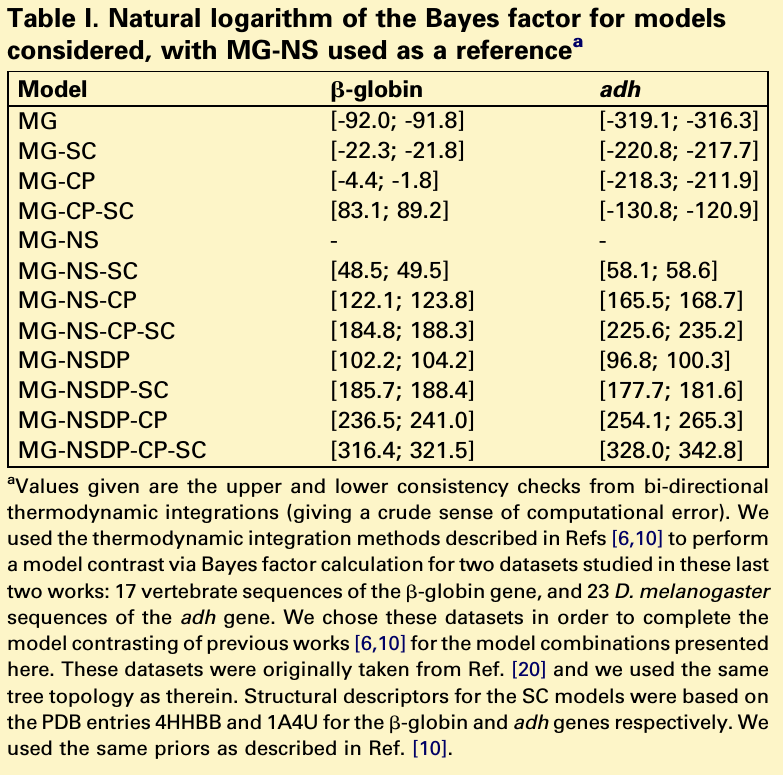
\includegraphics[scale=0.3]{Table1.png}
\end{center}

\begin{flushleft}
 \tiny{\cite{Rodrigue10b}}
\end{flushleft}
 \normalsize
}

%%%%%%%%%%%%%%%%%%%%%%%%%%%%%%%%%%%%%%%%%%%%%%%%%%%%%%%%%%%%%%%%%%%%%%%%%%%%%%%
\frame{
\frametitle{Still to be worked on}
\scriptsize
\begin{itemize}
 \item Zaheri, M.; Dib, L. \& Salamin, N. A generalized mechanistic codon model Molecular biology and evolution, 2014, 31, 2528-41
 \item Rodrigue, N. On the statistical interpretation of site-specific variables in phylogeny-based substitution models. Genetics, 2013, 193, 557-64
 \item Lartillot, N. \& Philippe, H. A Bayesian mixture model for across-site heterogeneities in the amino-acid replacement process. Molecular biology and evolution, 2004, 21, 1095-109
 \item Goldman, N., and Z. Yang, 1994 A codon-based model of nucleotide substitution for protein-coding DNA sequences. Mol. Biol. Evol. 11: 725–736.
 \end{itemize}
\normalsize
}

%%%%%%%%%%%%%%%%%%%%%%%%%%%%%%%%%%%%%%%%%%%%%%%%%%%%%%%%%%%%%%%%%%%%%%%%%%%%%%%
\frame[allowframebreaks]{  
\tiny \bibliography{../../phylo-models.bib}
\bibliographystyle{apalike}          % Style BST file
}


%%%%%%%%%%%%%%%%%%%%%%%%%%%%%%%%%%%%%%%%%%%%%%%%%%%%%%%%%%%%%%%%%%%%%%%%%%%%%%%%
\end{document}


%%%% unused %%%%%

%%%%%%%%%%%%%%%%%%%%%%%%%%%%%%%%%%%%%%%%%%%%%%%%%%%%%%%%%%%%%%%%%%%%%%%%%%%%%%%
%\frame{
%\frametitle{Multinomial distribution}
%The multinomial is a multivariate generalization of the Binomial and gives the distribution of counts over $m_{k}$.

%\begin{align}
%\text{Mult}(m_{1},\ldots,m_{K}|\bm{\mu},N) &= \binom{N!}{m_{1},\ldots,m_{M}} \prod^{M}_{k=1} \mu_{k}^{m_{k}}\\
%\mathbb{E}[m_{k}] &= N \mu_{k}\\
%\textrm{var}[m_{k}] &= N \mu_{k}(1-\mu_{k})\\
%\textrm{cov}[m_{j},m_{k}] &= -N \mu_{j} \mu_{k}
%\end{align}
%}

%%%%%%%%%%%%%%%%%%%%%%%%%%%%%%%%%%%%%%%%%%%%%%%%%%%%%%%%%%%%%%%%%%%%%%%%%%%%%%%
%\frame{
%\frametitle{Dirichlet distribution}
%\scriptsize
%Is a multivariate distribution over $K$ random variables $0 \leq \mu_{k} \leq 1$, where $k=1,\ldots,K$. Also, $\sum_{k} x_{k} = 1$, $\bm{\mu} = (\mu_{1},\ldots,\mu_{k})^{\textrm{T}}$ and %$\bm{\alpha} = (\alpha_{1},\ldots,\alpha_{k})^{\textrm{T}}$

%\begin{align}
%\textrm{Dir}(\bm{\mu}|\bm{\alpha}) &= \textrm{C}(\bm{\alpha}) \prod^{K}_{k=1} \mu_{k}^{\alpha_{k-1}}\\
%\mathbb{E}[x_{k}] &= \frac{\alpha_{k}}{\alpha}\\
%\end{align}

%Also, note that $\textrm{C}(\bm{\alpha}) \frac{\Gamma(\hat{\alpha})}{\Gamma(\alpha_{1}) \ldots \Gamma(\alpha_{K})}$ and $\hat{\alpha} = \sum^{K}_{k=1} \alpha_{k}$
%The Dirichlet forms the conjugate prior for the multinomial distribution and represents a generalization of the beta distribution.  $\alpha_{k}$ can be interpreted as the effective number of %observations of the corresponding values of the $K$-dimensional binary observation vector.
%\normalfont
%}
